%TODO: refer to grid convolutions as discrete (?)


\chapter{Artificial Neural Networks}
\label{chap:neuralnetworks}

\textit{Feed forward artificial neural networks}, or less formally, \textit{neural networks}, are a class of machine learning algorithm which are loosely inspired by neuroscientific models of how biological neural networks operate\cite{mcculloch1943}. 
Like many machine learning methods, a neural network is a parameterized function with vector input and either scalar or vector output.
For example, the input may be pixel intensities from an image of interest, and the output may be an integer corresponding to a label which indicates the image's content.
In this thesis, the function is denoted $f(x|\Theta)$, where $x$ is the input vector and $\Theta$ is the complete set of parameters, or weights.
In neural networks, $f$ is composed of a sequence of layers, $h_i(x_i|\Theta_i)$ which perform comparatively simple mathematical operations on their input to produce a layer output.
By convention, the input vector is considered the first layer of a neural network, even though it performs no operations, and the output of the last layer is the output of the entire network.
All intermediate layers are termed \textit{hidden layers}, each of which accepts the output of the preceding layer and passes its output to the subsequent layer.
The number of layers in a neural network (besides the first layer) is its \textit{depth}, and the number of outputs of a given layer is the number of \textit{units} (or \textit{neurons}) in that layer.
Figure \ref{fig:twolayernetwork} depicts a two layer neural network with three inputs, four units in the hidden layer, and two outputs.

\begin{figure}
	\centering
	%\begin{center}
	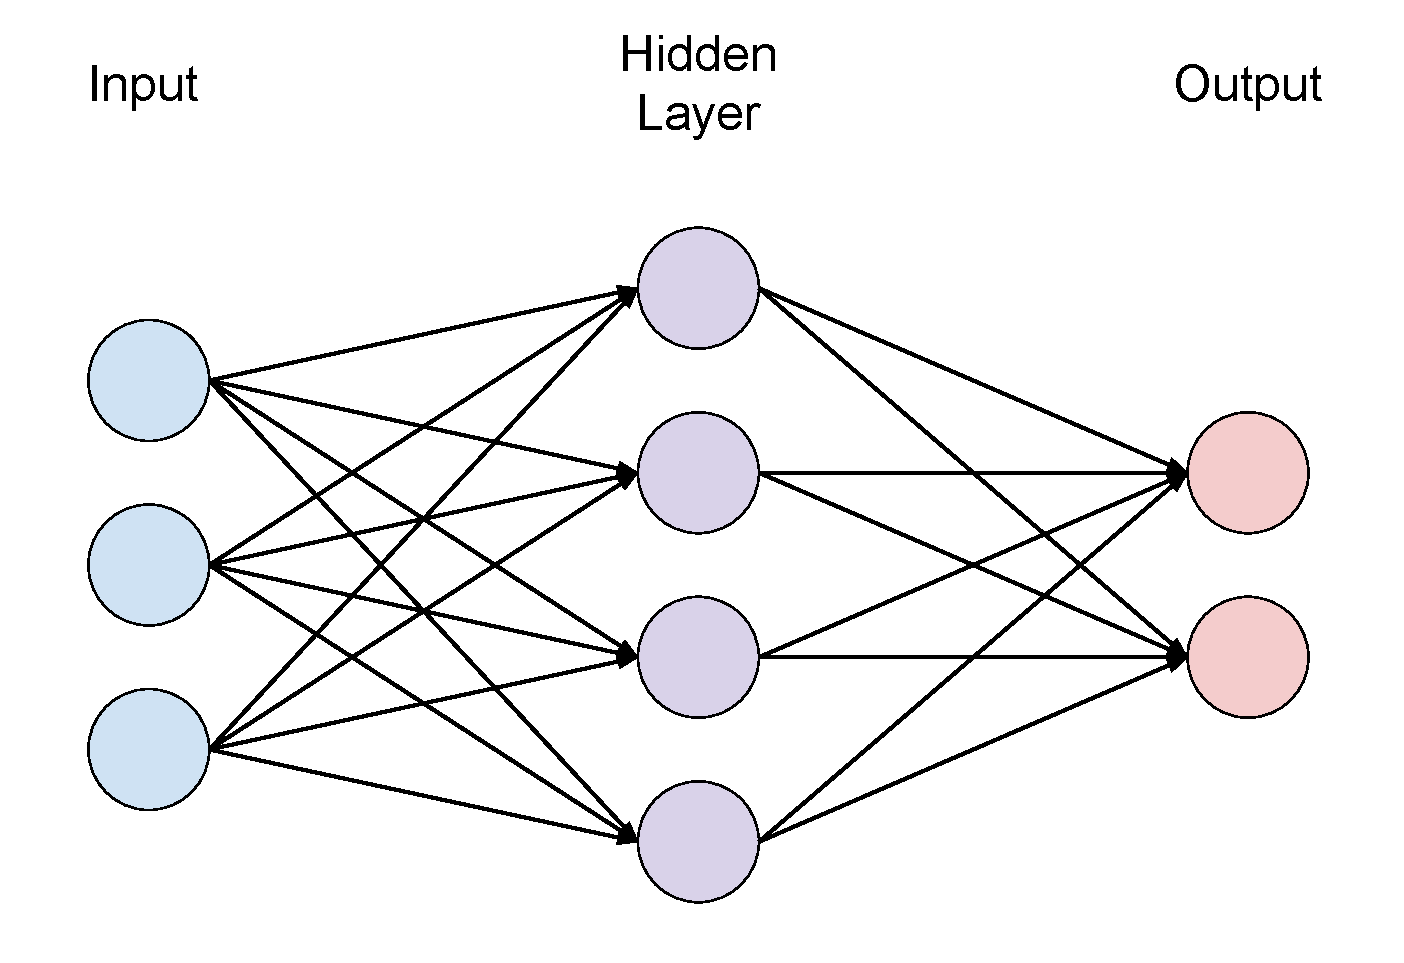
\includegraphics[width=0.8\textwidth]{twolayernetwork.pdf}
	%\end{center}
	\caption{A two layer neural network with a single hidden layer.}
	\label{fig:twolayernetwork}
\end{figure}

A common form of hidden layer is a \textit{dense layer}, in which each unit calculates a weighted sum of the layer inputs, where the set of weights is unique to each unit.
It is also common to add a scalar bias term and apply a nonlinear activation function to the weighted sum.
Dense layers have a convenient mathematical representation:

\begin{equation}
h(x|W, b)=\sigma(W x^T + b),
\label{eq:denselayer}
\end{equation}

\noindent
where $W$ is a matrix of weights, $x$ is the layer input, $b$ is a vector of biases, and $\sigma(\cdot)$ is a nonlinear activation function.
If there are $n$ inputs to a layer and $m$ units in the layer, then $W\in\mathbb{R}^{nxm}$ and $b\in\mathbb{R}^{m}$.
The expression $W x^T + b$ is called the \textit{signal}, and $h$ the \textit{activation}.
For hidden layers, activations have traditionally taken the form of a sigmoidal, or "s-shaped", function such as the logistic function, $\sigma(x) = 1/(1+e^{-x})$, or hyperbolic tangent, $\sigma(x) = tanh(x)$.

Despite being conceptually simple, this formulation of artificial neural networks is capable of approximating any continuous function on a compact subset in $\mathbb{R}$ with arbitrarily small error~\cite{cybenko1989}.
The challenge of using neural networks for function approximation is in finding the appropriate set of parameters to approximate the desired function.
For simple feed forward neural networks, this is accomplished by quantifying the error between the desired function and the approximation for a given training data set $X=(x_1, x_2, ..., x_N)$, using a differentiable loss function $L(\Theta | X)$. 
The weights are updated by differentiating $L$ with respect to $\Theta$ and "taking a step" in parameter space opposite the direction of the gradient. 
This update step can be repeated iteratively in a process called \textit{gradient descent}, which can be dated back to Augustin-Louis Cauchy~\cite{cauchy1847}.
Mathematically, 
\begin{equation}
\Theta_{k+1} = \Theta_k - \eta \nabla L(\Theta_k | X) = \Theta_k - \eta \sum_{n=1}^{N} \nabla L(\Theta_k | x_n),
\label{eq:batch_gd}
\end{equation}

\noindent
where $\eta$ is a tunable step size and $k$ indicates the iteration.
The gradient can be efficiently calculated using automatic differentiation~\cite{linnainmaa1976}, in which the update step is referred to as \textit{backpropagation}.
Weights are usually initialized by drawing from distributions that have some empirical or theoretical justification~\cite{glorot2010}.
A variant of this algorithm, called stochastic gradient descent (SCG) performs an update using a gradient computed from a random sample of the training data at each iteration.
There is also a batched version where the training data are randomly shuffled and divided into a fixed number of equal sized \textit{mini-batches} and an update is performed on each one. 
When all mini-batches have been used in an update step, this constitutes an \textit{epoch}.
Gradient descent is a first order method, however various second order methods have also been used to train neural networks~\cite{fletcher1964, polak1969, moller1993, marquardt1963}.

Like many machine learning algorithms, neural networks risk \textit{overfitting}, in which the network learns to approximate the training data (which usually contain noise), rather than the underlying function from which the training data are assumed to be drawn.
This hinders the ability of neural networks to generalize to unseen data.
In neural networks, overfitting is commonly the result of an overcomplete parameterization coupled with overtraining~\cite{reed1993, dalianis1993}.
Many regularization techniques have been introduced to prevent overfitting of neural networks, including early stopping~\cite{morgan1990}, model pruning~\cite{reed1993}, weight decay\cite{krogh1992}, lateral inhibition~\cite{krizhevsky2012}, induced sparsity~\cite{ng2011, makhzani2015}, and dropout~\cite{srivastava2014}, with dropout being one of the most common. 
Dropout consists of randomly dropping units from the neural network during the training phase.
Each time a training example is presented to the network, each unit in the network is dropped with probability $p$, commonly 0.5.
Each application of dropout can be seen as generating a new network whose units are a subset of the units in the original network.
Given $n$ units in a network, there are $2^n$ possible dropout networks all with a high degree of weight sharing.
During testing, no dropout is performed, and weights are rescaling by $p$.
This has the effect of averaging the prediction of each dropout network.
Dropout helps prevent overfitting by limiting the effective number of parameters in each dropout network and reducing the amount of co-adaptation among units in the network.\cite{srivastava2014}.


In recent years, more advanced forms of neural networks under the moniker \textit{deep learning} have demonstrated success in sophisticated tasks, particularly for image and speech recognition~\cite{krizhevsky2012, lecun2015, masci2011, hinton2012, he2016}, but also in a variety of other applications such as quantitative structure activity relationship (QSAR) prediction~\cite{ma2015}, particle detection~\cite{ciodaro2012}, and reinforcement learning\cite{mnih2015}.
These advances were catalyzed by the availability of large volumes of labeled data\cite{deng2009, krizhevsky2009} and the improvements in computing power from general purpose graphical processing units (GP-GPUs) and distributed systems\cite{chetlur2014, chu2007}.
Such factors allow experimentation with larger networks and more complicated layer operations such as convolutions, which are described in the following section.

\section{Convolutional Neural Networks}

Traditionally, neural networks do not explicitly account for inherent structure in the input which may be useful when approximating the output function.
For example, pixels in an image are often spatially correlated, but spatial information is not explicitly given to the network when using dense layers.
Convolutional layers are one way to incorporate structure information in a neural network. 
The name comes from an interpretation of how they operate on a set of inputs with a well defined grid structure, such as a pixelated image or discrete time series, where a filter of weights (e.g. 3x3 pixels for images) is convolved over the input grid.
That is, at each filter position, the filter weights are multiplied with the corresponding inputs, called the \textit{receptive field}, and summed to produce a scalar value.
As with dense layers, the result is usually passed through an activation function.
Because each filter multiplication is associated with a position of the input grid, the output retains a grid structure.
Figure \ref{fig:convolutionallayer} depicts a simple convolutional layer.
In color images, each pixel has multiple values, or \textit{channels}, which capture color information, and the filter must have the same number of channels as the input in order to take the elementwise product between the filter and the receptive field.
A convolutional layer may contain multiple filters, each of which produces a grid of scalar values which can be considered a channel in the output.
The weights in a filter determine which receptive fields produce a larger output and which do not, so a filter can be viewed as detecting specific patterns in a receptive field.
An alternate interpretation of convolutional layers is that weights are being shared across a layer such that each unit in the convolutional layer receives inputs from a different localized region of the input, and that all units share weights appropriately.

%TODO: equation?

\begin{figure}
	\centering
	%\begin{center}
	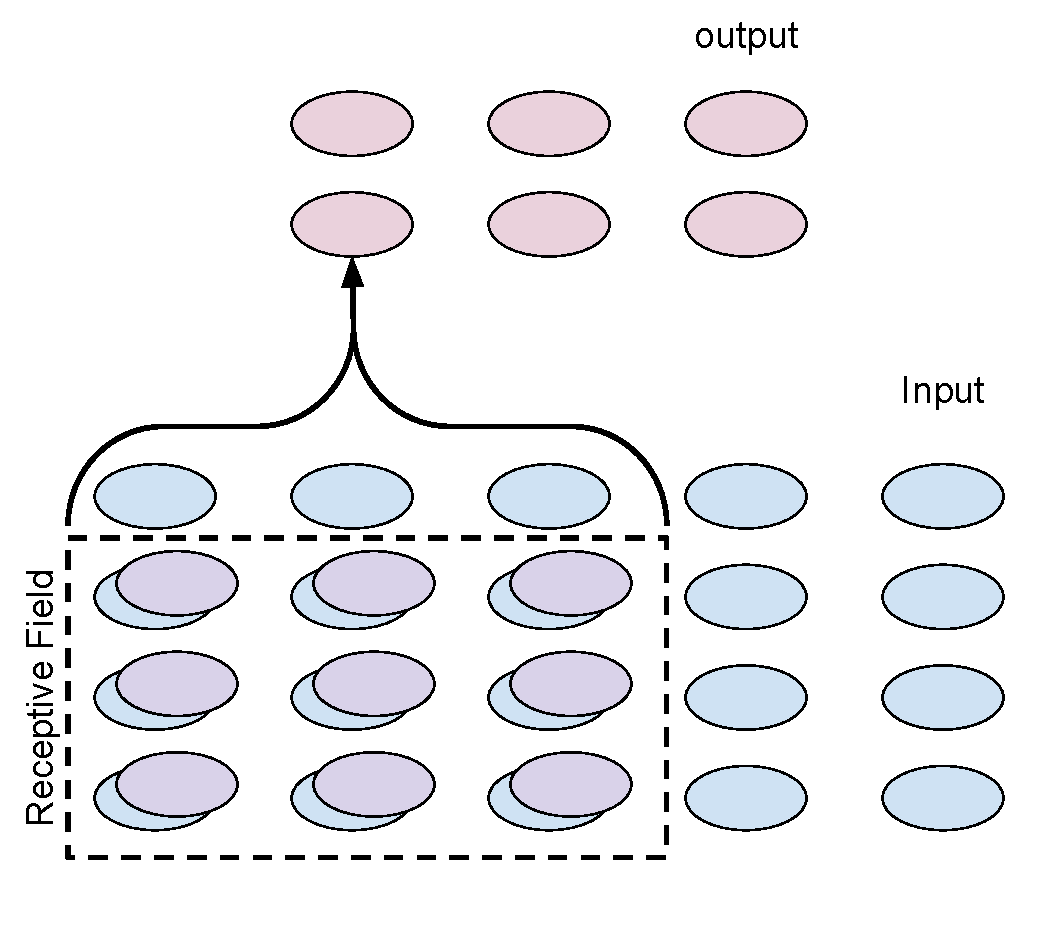
\includegraphics[width=0.8\textwidth]{convolutionallayer.pdf}
	%\end{center}
	\caption{A convolutional layer with a single 3x3 filter operating on a grid input with a single channel. The filter is multiplied elementwise with the corresponding inputs and produces a scalar value.}
	\label{fig:convolutionallayer}
\end{figure}


Convolutional layers exhibit certain properties which aid in image related tasks:
\begin{itemize}
\item
\textit{Local pattern detection}: Convolutional filters are usually significantly smaller than the size of the input, so for any given position of the filter they are operating on a local neighborhood of the input. 
This means that patterns detected by a particular filter are local.
\item
\textit{Translational Invariance}: Since filters are convolved over the input, patterns can be efficiently detected regardless of where they occur in the input.
In a dense layer, detection of a local pattern in each part of the input requires that weights associated with each region of the input be trained individually to detect the same pattern.
This means the training data must represent the same pattern in all portions of the input. 
For example, to train a dense layer to detect a cat's ear regardless of where it appears in an image, it must be trained using data which represent a cat's ear in every possible position in the image.
\item
\textit{Stackability}: The output of a convolutional layer retains the same grid structure as the input, so the output of a convolutional layer can be used as input to another convolutional layer.
Consider a neural network with two convolutional layers stacked on top of one another.
The receptive field of a unit in the second layer consists of units in the preceeding convolutional layer, each of which has its own receptive field in the input.
Hence filters in the second layer detect patterns of patterns in the original input, which suggests that stacked layers learn a hierarchical representation of the original input.
Furthermore, stacked layers have effectively larger receptive fields on the original input, and are therefore able to detect larger patterns in the original input.
The ability to learn a conceptual hierarchy of patterns in the input, from simple textures and edges to complex objects like faces or vehicles, has been demonstrated empirically as well~\cite{zeiler2013}.
\item
\textit{Robustness to overfitting}: The weight sharing inherent in convolutional layers means there are fewer trainable weights compared to a dense layer with the same number of hidden units. 
This reduces the propensity of the network to overfit to the training data and improves its ability to generalize to unseen examples.
\end{itemize}

Convolutional neural networks often incorporate \textit{pooling layers}, which reduce a small region of a grid (e.g. 2x2 pixels for an image) to a single grid element that takes either the maximum or average value (per channel) of the region. 
Pooling allows downsampling of the grid, and is often performed between convolutional layers. 

The convolutions described above can only operate on a regular grid. 
Proteins, however, have inherently irregular structure. 
In this work the notion of convolution to work with irregular structure, which are represented as graphs, as described in Chapter \ref{chap:methods}.





